\documentclass[a4paper,12pt]{article}
\usepackage[utf8]{inputenc}
\usepackage{graphicx}
\usepackage{amsmath}
\usepackage{algorithm}
\usepackage{algorithmic}
\usepackage{hyperref}
\usepackage[T1]{fontenc}
\usepackage{pgfplots}

\title{Laboratory paper}
\author{Barbu David Constantin
Grupa 1, Anul 1, Secțiunea Calculatoare (engleza)}

\begin{document}

% Coperta
\begin{titlepage}
    \centering
    \vspace*{1cm}
    
    \Huge
    \textbf{Laboratory Paper}
    
    \vspace{2cm}
    
    \LARGE
    Barbu David Constantin \\
    Grupa 1, Anul I, Secțiunea Calculatoare (engleza)
    
    \vfill
    
\end{titlepage}

\newpage

% Cuprins
\tableofcontents
\href{http://www.example.com}{Link GitHub}
\newpage

% Secțiuni
\section{Problem statement}
The purpose of this lab work is to solve the following problem: a fisherman must choose from a set of lobsters those with the maximum sum of their values, but with a sum of dimensions smaller than the capacity of his net. The problem differs from the classic knapsack problem in that the chosen lobsters must be enumerated.

Specifically, it is considered that the fisherman has a net with a given maximum capacity. He has at his disposal an undetermined number of lobsters, each associated with three essential characteristics: name, size, and value. The program should receive as input the maximum capacity of the net and detailed information about each lobster. The objective is to determine the optimal combination of lobsters that maximizes the total value, while respecting the capacity constraint of the net.

The formulation of the problem can be presented mathematically as follows:

\begin{itemize}
    \item \textbf{Input}:
    \begin{itemize}
        \item \( C \) - the maximum capacity of the net (a positive constant).
        \item \( n \) - the number of available lobsters.
        \item For each lobster \( i \) (\( i = 1, 2, \ldots, n \)):
        \begin{itemize}
            \item \( \text{name}_i \) - the name of lobster \( i \) (a string of characters).
            \item \( \text{size}_i \) - the size of lobster \( i \) (a positive real number).
            \item \( \text{value}_i \) - the value of lobster \( i \) (a positive real number).
        \end{itemize}
    \end{itemize}
    \item \textbf{Output}:
    \begin{itemize}
        \item A subset of selected lobsters such that:
        \begin{itemize}
            \item The sum of the sizes of the selected lobsters is less than or equal to \( C \).
            \item The sum of the values of the selected lobsters is maximum.
            \item The selected lobsters are enumerated.
        \end{itemize}
    \end{itemize}
\end{itemize}

Thus, the problem falls into the class of combinatorial optimization problems, being a variation of the knapsack problem, but with an additional requirement to enumerate the selected lobsters. Implementing an efficient algorithm for this problem will need to consider combinatorial complexity, ensuring that the obtained solution is optimal given the constraints provided.

\section{Algorithms}
\subsection{Algoritm rucsac}
In order to get the maximum possible value that can fit in the net I used the knapsack dynamic programming algorithm. The time complexity is O(n * c) where n is the number of lobsters and c the maximum capacity.
\begin{algorithm}
\caption{(Knapsack)}
\begin{algorithmic}[1]

\STATE \text{Let a table } \( K[0..n][0..C] \)
\FOR {i = 0 \TO n}
    \FOR {cap = 0 \TO C}
        \IF {i == 0 \OR cap == 0}
            \STATE \( K[i][cap] = 0 \)
        \ELSIF {w[i] \text{<=} cap}
            \STATE \( K[i][cap] = \max(v[i] + K[i-1][cap-w[i]], K[i-1][cap]) \)
        \ELSE
            \STATE \( K[i][cap] = K[i-1][cap] \)
        \ENDIF
    \ENDFOR
\ENDFOR
\STATE \textbf{return} \( K[n][C] \)
\end{algorithmic}
\end{algorithm}

\subsection{Explanation of the knapsack algorithm}

Let's detail the steps of the algorithm:

\begin{itemize}
    \item We define a table \( K \) where \( K[i][cap] \) represents the maximum value that can be obtained using the first \( i \) objects and having the capacity \( cap \) available in the knapsack.
    \item We initialize the table \( K \) with zero for base cases where either the number of objects is zero, or the knapsack capacity is zero.
    \item For each object \( i \) and each capacity \( cap \):
    \begin{itemize}
        \item If the size of object \( i \) is less than or equal to the capacity \( cap \), then we have two options:
        \begin{itemize}
            \item Include object \( i \) and add its value to the optimal value of the knapsack with remaining capacity \( cap - w[i] \).
            \item Do not include object \( i \) and take the optimal value of the knapsack without this object.
        \end{itemize}
        \item We choose the option that offers the maximum value.
        \item If the size of object \( i \) is greater than the capacity \( cap \), we cannot include the object, so we keep the optimal value without this object.
    \end{itemize}
    \item The final result, i.e., the maximum value that can be obtained with capacity \( C \) using all the objects, is found in \( K[n][C] \).
\end{itemize}

\subsection{Algorithm for enumerating selected items}

To determine which objects have been selected to achieve the maximum value, we can traverse the table \( K \) in reverse order, starting from \( K[n][C] \):

\begin{algorithm}
\caption{Algorithm for Enumerating Selected Items}
\begin{algorithmic}[1]

\STATE \text{Initialize the empty list } \text{selectedItems}
\STATE \( \text{cap} = C \)
\FOR {i = n \TO 1 \text{ with step } -1}
    \IF {K[i][\text{cap}] \text{!=} K[i-1][\text{cap}]}
        \STATE \text{Add object } i \text{ to } \text{selectedItems}
        \STATE \( \text{cap} = \text{cap} - w[i] \)
    \ENDIF
\ENDFOR
\STATE \textbf{return} \text{selectedItems}
\end{algorithmic}
\end{algorithm}

\subsection{Explanation of the Algorithm for Enumerating Selected Items}

The algorithm for enumerating selected items utilizes the table \( K \) to identify the objects included in the optimal solution:

\begin{itemize}
    \item We start from position \( K[n][C] \) and check if the current value differs from the one above it \( K[i-1][cap] \).
    \item If the values are different, it means object \( i \) was included in the knapsack. We add the object to the list of selected items and decrease the available capacity \( cap \) by the size of object \( i-1 \).
    \item We continue this process until we reach the first object.
    \item The resulting list, \text{selectedItems}, contains the objects that were included to achieve the maximum value.
\end{itemize}

The complexity of the enumeration algorithm is O(number of objects), so it does not affect the overall program complexity.


\section{Experimental Data}

The program was ran on ten test files. Each test file was randomly generated using the "test-generator" program. The data had lobsters with names less than 100 charachter, with sizes and values in between 1 and 1000.
The first test file has 1000 lobsters and 1000 maximum bag capacity. It then grows by 1000 for every test file. The parametres used for generating the files can be found in the params folder. The same test files were used for testing both the C and Python implementation.
Both implementations produced the same results.

Here is a graph mapping the C implementation execution time to the number of objects in each test case.	

\begin{figure}[h]
  \centering
  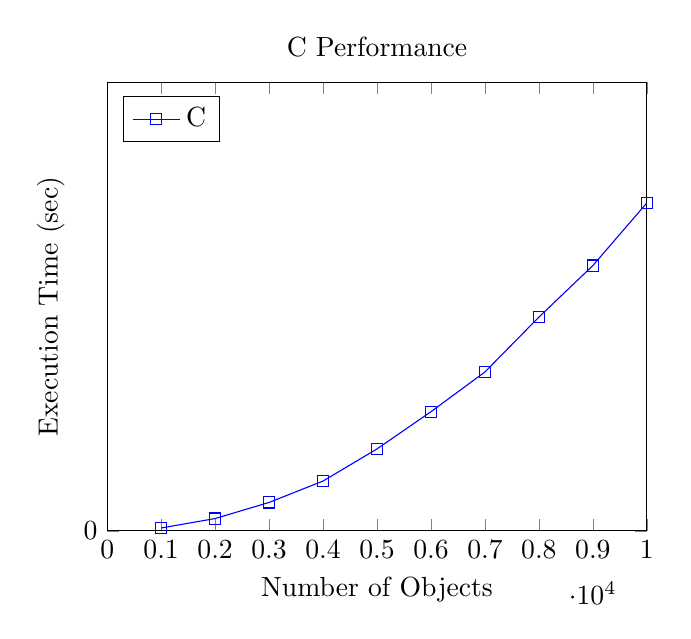
\begin{tikzpicture}
    \begin{axis}[
        xlabel={Number of Objects},
        ylabel={Execution Time (sec)},
        title={C Performance},
        xmin=0, xmax=10000,
        ymin=0, ymax=3,
        xtick={0,1000,2000,3000,4000,5000,6000,7000,8000,9000,10000},
        ytick={0,20,40,60,80,100,120},
        legend pos=north west,
        ymajorgrids=true,
        grid style=dashed,
      ]
      
      \addplot[
        color=blue,
        mark=square,
      ]
      coordinates {
        (1000,0.019)(2000,0.082)(3000,0.190)(4000,0.333)(5000,0.548)(6000,0.797)(7000,1.063)(8000,1.430)(9000,1.775)(10000,2.194)
      };
      \legend{C}
      
    \end{axis}
  \end{tikzpicture}
\end{figure}

The execution time grows exponentially, because the time complexity is O(n*c), and here c is equal to n. The same is true of the Python implementation, but it is much slower (50x).

\begin{figure}[h]
  \centering
  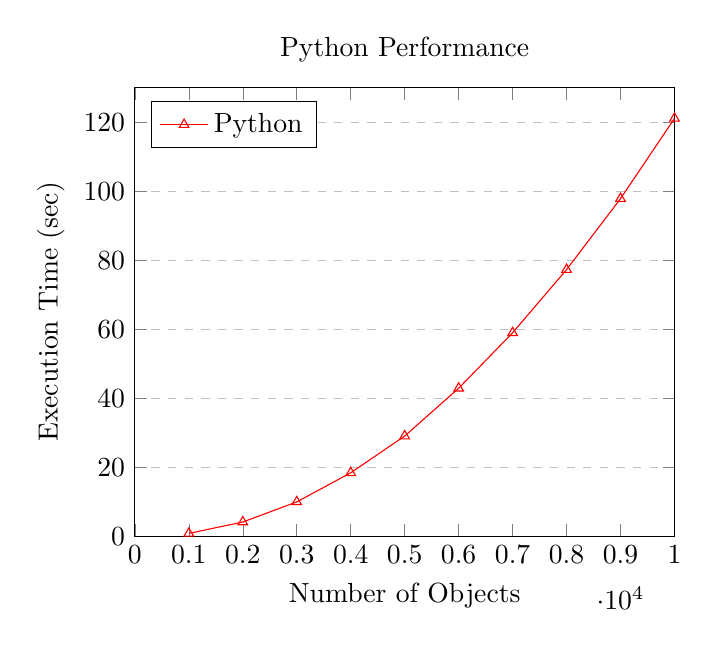
\begin{tikzpicture}
    \begin{axis}[
        xlabel={Number of Objects},
        ylabel={Execution Time (sec)},
        title={Python Performance},
        xmin=0, xmax=10000,
        ymin=0, ymax=130,
        xtick={0,1000,2000,3000,4000,5000,6000,7000,8000,9000,10000},
        ytick={0,20,40,60,80,100,120},
        legend pos=north west,
        ymajorgrids=true,
        grid style=dashed,
      ]
      
      \addplot[
        color=red,
        mark=triangle,
      ]
      coordinates {
        (1000,0.811)(2000,4.108)(3000,9.936)(4000,18.381)(5000,29.041)(6000,42.897)(7000,58.982)(8000,77.308)(9000,97.888)(10000,121.142)
      };
      \legend{Python}
      
    \end{axis}
  \end{tikzpicture}
\end{figure}
\newpage

The next graph compares the C and Python implementations.
\begin{figure}[h]
  \centering
  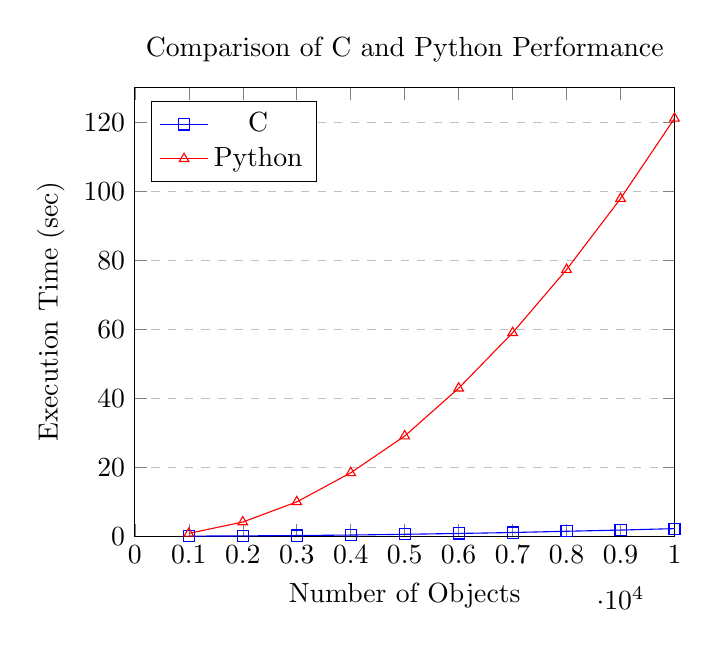
\begin{tikzpicture}
    \begin{axis}[
        xlabel={Number of Objects},
        ylabel={Execution Time (sec)},
        title={Comparison of C and Python Performance},
        xmin=0, xmax=10000,
        ymin=0, ymax=130,
        xtick={0,1000,2000,3000,4000,5000,6000,7000,8000,9000,10000},
        ytick={0,20,40,60,80,100,120},
        legend pos=north west,
        ymajorgrids=true,
        grid style=dashed,
      ]
      
      \addplot[
        color=blue,
        mark=square,
      ]
      coordinates {
        (1000,0.019)(2000,0.082)(3000,0.190)(4000,0.333)(5000,0.548)(6000,0.797)(7000,1.063)(8000,1.430)(9000,1.775)(10000,2.194)
      };
      \addlegendentry{C}
      
      \addplot[
        color=red,
        mark=triangle,
      ]
      coordinates {
        (1000,0.811)(2000,4.108)(3000,9.936)(4000,18.381)(5000,29.041)(6000,42.897)(7000,58.982)(8000,77.308)(9000,97.888)(10000,121.142)
      };
      \addlegendentry{Python}
      
    \end{axis}
  \end{tikzpicture}
\end{figure}
 
\newpage
\section{Tools used}

All of the tools I used during the development of this program are free and open source. For builiding the project I used the make utility with the gcc compiler, and for writing, vim, a text editor. Th OS used was Arch Linux, also FOSS. During development I ran into runtime errors, and I used Valgrind for debugging. For writing the report Latex was used because it is plainly better than proprietary alternatives like Microsof Word.


\section{Results and conclusions}

My findings confirm the correctness of the algorithm across all tested scenarios, demonstrating its reliability and robustness in producing accurate results.
A detailed comparison between the C and Python implementations of the algorithm revealed significant insights. The C implementation, while more challenging and time-consuming to code due to its lower-level nature and stricter syntax, proved to be considerably faster in execution. This speed advantage makes C an ideal choice for performance-critical applications. Conversely, the Python implementation, characterized by its simplicity and ease of coding, albeit slower in execution, is more suitable for rapid development and prototyping where development time is a higher priority than execution speed.

The evaluation of software tools highlighted the superiority of Free and Open Source Software (FOSS) tools in terms of flexibility, cost-efficiency, and community support. These tools not only provided comprehensive functionalities but also facilitated easier integration and customization, making them preferable for both development and deployment.

A possible continuation of this project could involve implementing the algorithm in a functional programming language such as Haskell. This would provide an opportunity to compare the functional paradigm with the imperative nature of C and the object-oriented approach of Python, potentially uncovering new insights into the efficiency and expressiveness of different programming paradigms.

In conclusion, this report has demonstrated the algorithm's correctness and provided a comprehensive evaluation of different development tools and programming languages. The insights gained emphasize the strengths of FOSS tools and the trade-offs between coding ease and execution speed in C and Python.

\end{document}
